% Editable reconstruction; interpretation recorded in root.json.
% Shared standalone design for the editable figure reconstructions.
\documentclass[tikz,border=5pt,10pt]{standalone}
\usepackage[T1]{fontenc}
\usepackage[utf8]{inputenc}
\usepackage{newpxtext,newpxmath}
\usepackage[scaled=.94]{sourcesanspro}
\usepackage{pgfplots}
\pgfplotsset{compat=1.18}
\usetikzlibrary{arrows.meta,calc,positioning,decorations.pathreplacing,
  decorations.markings,patterns,matrix,shapes.geometric,fit,backgrounds,
  intersections,angles,quotes}
\definecolor{ink}{HTML}{203746}
\definecolor{accent}{HTML}{146C78}
\definecolor{muted}{HTML}{667780}
\definecolor{signalred}{HTML}{B94B44}
\color{ink}
\tikzset{>=Latex,line width=.8pt,
  every node/.style={font=\small},
  axis/.style={->,draw=muted,line width=.5pt},
  guide/.style={draw=muted,dashed,line width=.45pt},
  curve/.style={draw=accent,line width=1pt},
  marker/.style={circle,fill=accent,inner sep=1.5pt},
  labelbox/.style={fill=white,inner sep=2pt}}

\begin{document}

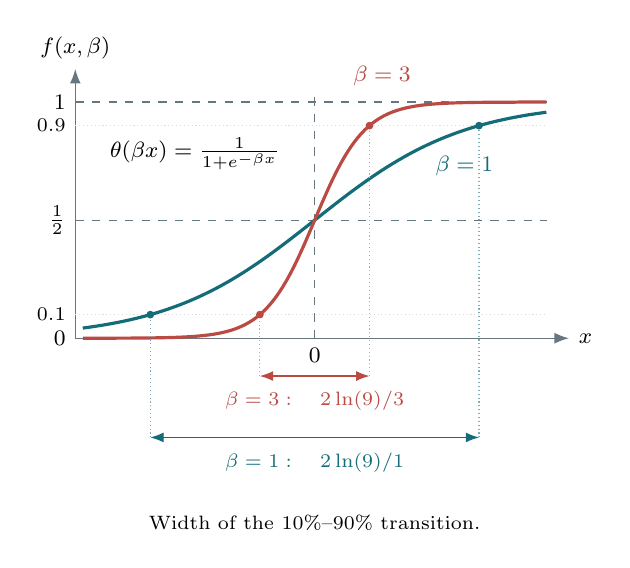
\begin{tikzpicture}[x=.95cm,y=3cm,every node/.style={font=\footnotesize}]
\draw[axis] (-3.2,0)--(3.4,0) node[right] {$x$};
\draw[axis] (-3.2,0)--(-3.2,1.14) node[above] {$f(x,\beta)$};
\draw[guide] (-3.2,1)--(3.1,1) (-3.2,.5)--(3.1,.5) (0,0)--(0,1.04);
\draw[muted!25,densely dotted] (-3.2,.1)--(3.1,.1) (-3.2,.9)--(3.1,.9);
\node[left,font=\scriptsize] at (-3.2,.1) {$0.1$};
\node[left,font=\scriptsize] at (-3.2,.9) {$0.9$};
\draw[accent,line width=1.15pt,domain=-3.1:3.1,samples=180] plot (\x,{1/(1+exp(-\x))});
\draw[signalred,line width=1.15pt,domain=-3.1:3.1,samples=180] plot (\x,{1/(1+exp(-3*\x))});
\node[left] at (-3.2,0) {$0$};\node[left] at (-3.2,.5) {$\frac12$};\node[left] at (-3.2,1) {$1$};\node[below] at (0,0) {$0$};
\node[accent,fill=white] at (2,.73) {$\beta=1$};\node[signalred,fill=white] at (.9,1.11) {$\beta=3$};
\node[align=center,fill=white,inner sep=2pt] at (-1.6,.78) {$\theta(\beta x)=\frac1{1+e^{-\beta x}}$};
% Each width uses the actual abscissae of the 0.1 and 0.9 crossings.
\foreach \b/\col/\height in {3/signalred/-.16,1/accent/-.42}{
  \draw[\col!55,densely dotted] ({-ln(9)/\b},\height)--({-ln(9)/\b},.1)
    ({ln(9)/\b},\height)--({ln(9)/\b},.9);
  \fill[\col] ({-ln(9)/\b},.1) circle(1.4pt);
  \fill[\col] ({ln(9)/\b},.9) circle(1.4pt);
  \draw[<->,\col] ({-ln(9)/\b},\height)--({ln(9)/\b},\height)
    node[midway,below=2pt,font=\scriptsize] {$\beta=\b:\quad 2\ln(9)/\b$};
}
\node[font=\scriptsize] at (0,-.78) {Width of the 10\%--90\% transition.};
\end{tikzpicture}
\end{document}
